\documentclass[conference]{IEEEtran}

% IEEEtran package options
%----------------------------------------------------------------------
% *** CITATION PACKAGES ***
\usepackage{cite}

% *** GRAPHICS RELATED PACKAGES ***
\usepackage[pdftex]{graphicx}
\graphicspath{{figures/}}
\DeclareGraphicsExtensions{.pdf,.eps}

% *** MATH PACKAGES ***
%\usepackage[cmex10]{amsmath}
%\interdisplaylinepenalty=2500

% *** SPECIALIZED LIST PACKAGES ***
%\usepackage{algorithmic}

% *** ALIGNMENT PACKAGES ***
%\usepackage{array}
%\usepackage{mdwmath}
%\usepackage{mdwtab}
%\usepackage{eqparbox}

% *** SUBFIGURE PACKAGES ***
%\usepackage[tight,footnotesize]{subfigure}
%\usepackage[caption=false,font=footnotesize]{subfig}

% *** FLOAT PACKAGES ***
%\usepackage{fixltx2e}
%\usepackage{stfloats}

% *** PDF, URL AND HYPERLINK PACKAGES ***
%\usepackage{url}
%----------------------------------------------------------------------



% added by Vaibhav
%----------------------------------------------------------------------
\usepackage[utf8]{inputenc}
\usepackage[nolist]{acronym}
\renewcommand{\ttdefault}{cmtt}

% temporaries
\usepackage{scrtime}
\usepackage{prelim2e}
\usepackage{todonotes}
\renewcommand{\PrelimWords}{\relax}
\renewcommand{\PrelimText}{\footnotesize[\,\today\ at \thistime\,]}
%----------------------------------------------------------------------

\begin{document}

\title{NFQL: The Swiss-Army Knife of Efficient Flow-Record Processing}

\author{\IEEEauthorblockN{Vaibhav Bajpai, Johannes Schauer, Jürgen
Schönwälder} \IEEEauthorblockA{School of Electrical and Computer Science\\
  Campus Ring 1, Jacobs University Bremen\\ \texttt{\{v.bajpai, j.schauer,
  j.schoenwaelder\}@jacobs-university.de} }}

\maketitle


\begin{abstract} Cisco's NetFlow protocol and IETF's IPFIX open standard have
  contributed heavily in pushing IP flow export as the de-facto technique for
  collecting aggregate network traffic statistics. These flow records have the
  potential to be used for billing and mediation, bandwidth provisioning,
  detecting malicious attacks and network performance evaluation. However,
  understanding certain traffic patterns requires sophisticated flow analysis
  tools that can mine flow records for such a usage. We recently proposed a
  flow query language that can cap such flow-records. In this paper, we
  introduce \ac{NFQL}. an efficient implementation of the query language.
  \ac{NFQL} can process flow records, aggregate them into groups, apply
  absolute (or relative) filters, invoke Allen interval algebra rules, and
  merge group records. The implementation has been evaluated by suite of
  benchmarks against contemporary flow-processing tools.\end{abstract}
% no keywords



\section{Introduction}
Researchers, service providers and security analysts have long been interested
in network and user behavioral patterns of the traffic crossing the internet
backbone. They want to use this information for the purpose of billing and
mediation, bandwidth provisioning, detecting malicious attacks, network
performance evaluation and overall improvement. Traffic measurement techniques
that have been rapidly evolving in the last decade have today matured enough
to provide such an insight.

Capturing network flow records has emerged out to be one of the favored
network measurement techniques. In this technique, packets traversing an
obvervation point are not captured raw, instead common characteristics of the
packet header are aggregated into flow records. They are then exported to a
collector for further analysis.  This reduces the amount of traffic aggregated
at the collector.

NetFlow and \ac{IPFIX} are the two popular protocols for IP flow information
export. NetFlow \cite{rfc3954} is a network protocol designed by Cisco
Systems, which allows routers to generate and export flow records to a
designated collector. NetFlow v$9$ provides flexibility through user-tailored
export templates, \ac{MPLS} and IPv$6$ support and a larger set of flow keys.
\ac{IPFIX} \cite{rfc5101} on the other hand is an open standard by IETF based
on NetFlow v$9$. The novelty of the standard lies in its ability to describe
record formats at runtime using templates based on an extensible and
well-defined information model. The data transfer mechanism is also simplistic
and extensible by being unidirectional and transport protocol agnostic.

The wide applicability of this approach is easily seen from the pervasive use
of flow records for a vibrant set of network analysis applications. For
instance, a survey by Sperotto \textit{et al.} \cite{sperotto:2010} gives an
overview of how network flow analysis can be used to detect Denial of Service
attacks, scan probing target systems and the target discovery phase of worms.
In addition, a survey by Callado \textit{et al.} \cite{callado:2009} also
lists behaviour analysis of Internet backbone traffic and general anomaly
detection.

Understanding intricate traffic patterns require sophisticated flow analysis
tools that can mine flow records for such a usage.  Unfortunately current
tools fail to deliver owing to their language design and simplistic filtering
methods.  We recently proposed a flow query language design
\cite{vmarinov:2009} that aims to cater to such needs.  It can process
flow records, aggregate them into groups, apply absolute or relative filters
and invoke Allen interval algebra rules \cite{fallen:1983}. The expressiveness
of the language can be seen from \cite{vperelman:2011} where the authors
formulate flow queries to identify flow signatures of popular applications.

Flowy \cite{kkanev:2010} was a first feature complete Python prototype of that
flow query language. Due to performance problems, it was superseeded by a
complete rewrite in C, called Flowy 2.0 \cite{jschauer:thesis:2011}. In this
paper, we introduce \ac{NFQL} which extends on Flowy 2.0, making it more
feature complete and optimizing its execution engine with crispier algorithms.
We show that this iteration of our work is able to scale to real-world sized
traces and has comparable execution times to contemporary flow analysis tools.

The paper is organized as follows. In section \ref{sec:relatedwork} we survey
the current state-of-the-art flow-processing tools and reason how \ac{NFQL} is
different from each one of them. In section \ref{sec:design} we describe the
flow query language by discussing each stage of the processing pipeline. In
section \ref{sec:implementation} we introduce the inner workings of \ac{NFQL}.
It begins by providing an overview of the \ac{NFQL} architecture and the
structure of the intermediate format used to exchange messages. The workflow of
the execution engine is described next and is supplemented by a number of
performance optimizations made to make the implementation scale. The section is
followed by performance evaluations comparing \ac{NFQL} against contemporary
flow processing tools alongwith with a discussion on its current limitation and
future outlook in section \ref{sec:evaluation}, with conclusion in section
\ref{sec:conclusion}.

\begin{figure*}[!t]
\centering
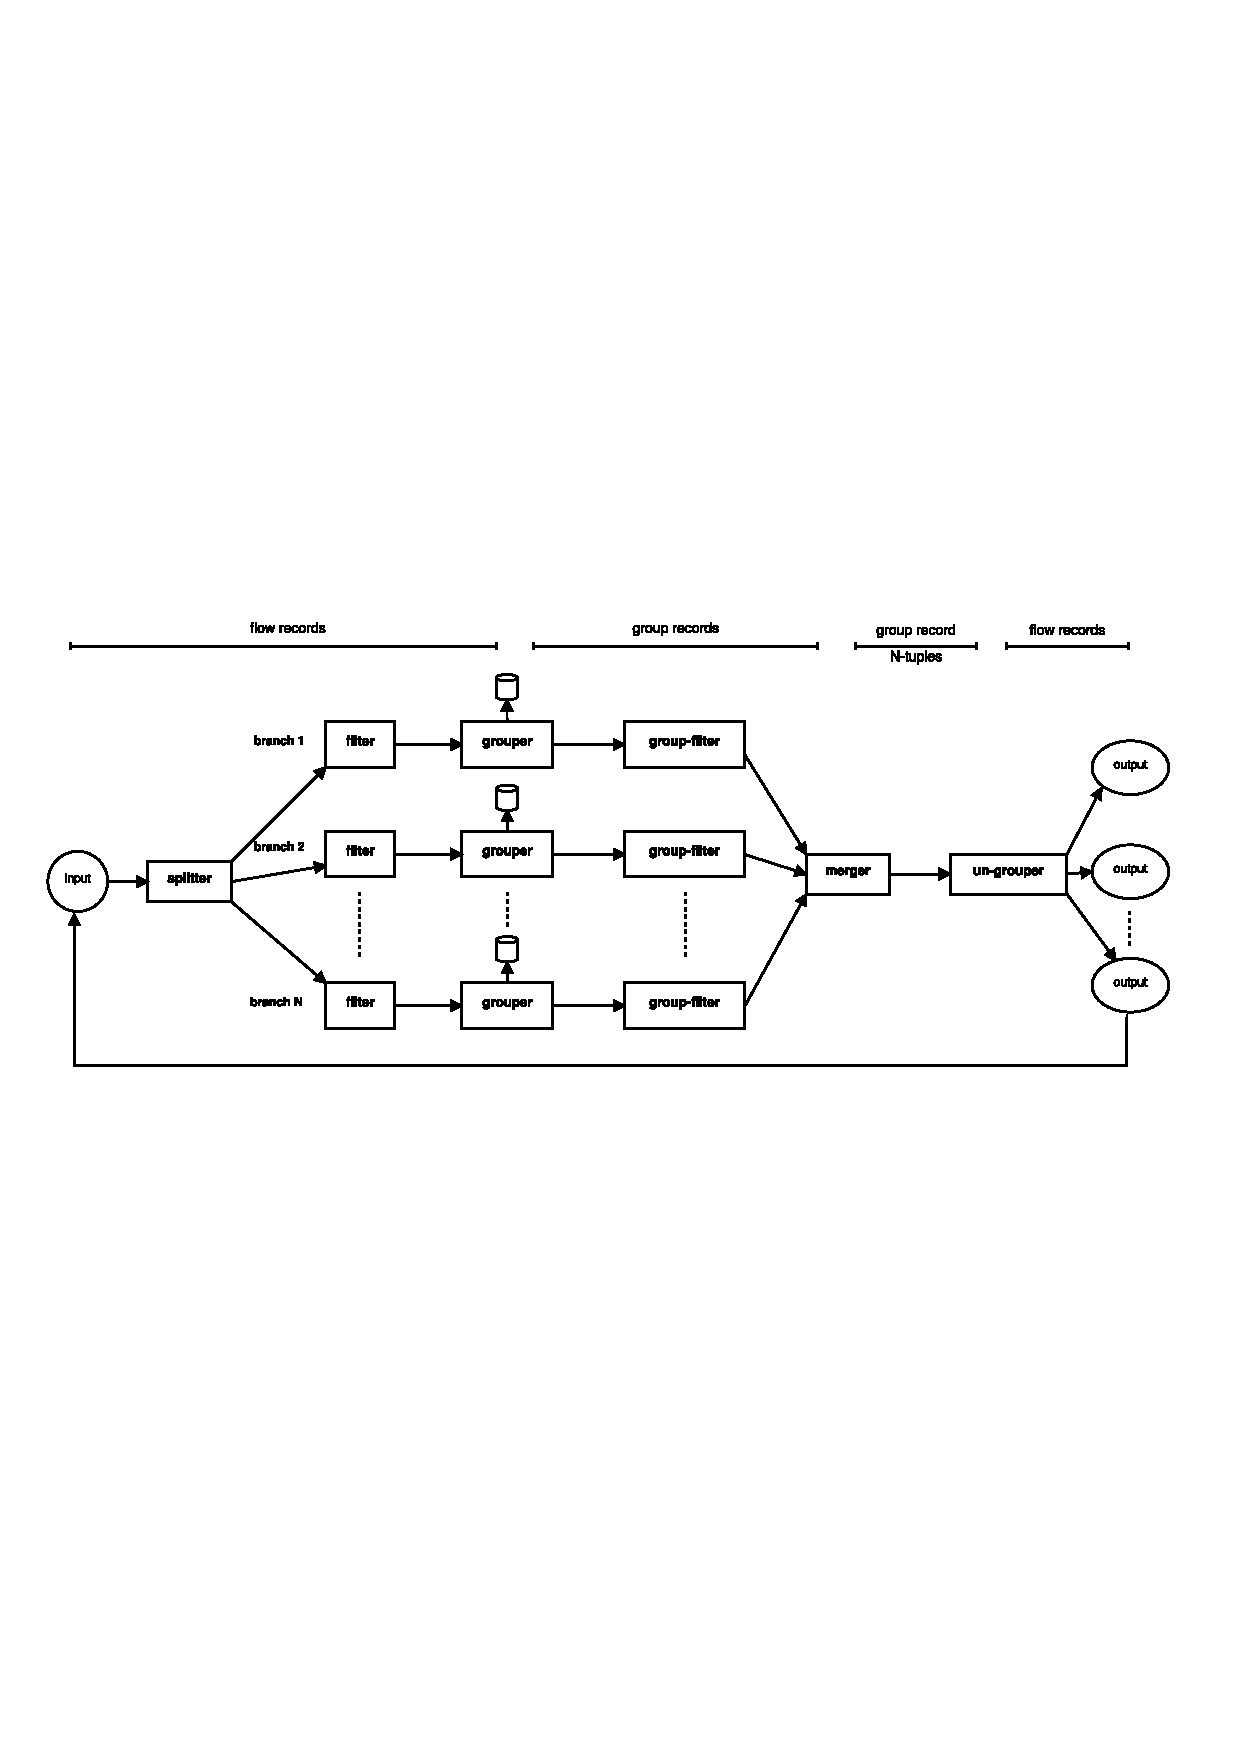
\includegraphics[width=0.9\linewidth]{nfql-pipeline}
\caption{NFQL Processing Pipeline \cite{vmarinov:2009}}
\label{fig:nfql-pipeline}
\end{figure*}

\section{Related Work}
%The study of the network traffic patterns began with tools that utilized raw
%packet captures at the monitoring point for traffic measurement.
%\texttt{tcpdump} and \texttt{wireshark} have since then become the de-facto
%tools for packet capture and analysis. \texttt{tcpdump} \cite{tcpdump-manpage}
%is a premier command-line utility that uses the \texttt{libpcap}
%\cite{pcap-manpage} library for packet capture. The power of \texttt{tcpdump}
%comes from the richness of its expressions, the ability to combine them using
%logical connectives and extract specific portions of a packet using filters.
%\texttt{wireshark} \cite{wireshark-manpage} is a GUI application, aimed at
%both journeymen and packet analysis experts. It supports a large number of
%protocols, has a straightforward layout, excellent documentation, and can run
%on all major operating systems.

In recent years, a number of tools have been developed that can capture the
traffic as flow records and use them for network analysis. \texttt{flow-tools}
and \texttt{nfdump} are among the most popular tools used for analyzing
NetFlow data. \texttt{flow-tools} \cite{sromig:2000} is a suite of programs
for capturing and processing NetFlow v5 flow records. It consists of 24
separate tools that work together by connecting them via UNIX pipes. It can
capture, read, filter, and print flow records internally saved in a fixed-size
format. \texttt{nfdump} \cite{phaag:2006} is a very similar tool that uses a
different storage format. Flow records are captured using \texttt{nfcapd} and
then processed by \texttt{nfdump}. The power of filtering rules in both the
tools is however mostly limited to absolute comparisons of flow attributes. As
a result, relative comparison amongst different flows or querying a timing
relationship among them is not possible.  SiLK \cite{SiLK} is a network
traffic collection and analysis tool developed and maintained by the CERT
Network Situational Awareness Team (CERT NetSA) at Carnegie Mellon University.
SiLK is the tool that comes quite close to providing similar capabilities as
provided by \ac{NFQL} and is therefore used as a reference point to compare
the performance of the \ac{NFQL} execution engine in this paper. The design
and implementation of SiLK, however, differs a lot from that of \ac{NFQL}. For
instance, in SiLK there are separate tools to perform the task of each stage
of the \ac{NFQL} processing pipeline. The stage functionality is not
full-fledged though. The grouping and merging operations can only be performed
using an equality operator. This restriction allows the tool to perform
optimization such as using hash tables to perform lookups. There are also
stringent requirements to how flow-data needs to be organized before it can be
piped into a tool. The grouping tool, for instance, assumes that the to-be
supplied input flow data is already sorted on the field column.  These
requirements can make it a little cumbersome to design a full-fledged flow
query.  For instance, trying to mimic a \ac{NFQL} query in SiLK sometimes ends
up as a shell script with over a dozen of SiLK tools piped together.

\section{Flow Query Language}
The flow query language pipeline consists of a number of independent elements
that are connected to one another using UNIX-based pipes.  Each element
receives the content from the previous pipe, performs an operation and pushes
it to the next element in the pipeline as shown in Fig.
\ref{fig:nfql-pipeline}. A complete description on the semantics of each
element in the pipeline can be found in \cite{vmarinov:2009}

The pipeline starts with the splitter. It takes the flow-records data as input
in the \texttt{flow-tools} compatible format. The splitter is responsible to
duplicate the input data out to several branches without any processing
whatsoever. This allows each of the branch to receive an identical copy of the
flow data to process it independently.

The filter is the first processing element of a branch in the pipeline.  It
performs \emph{absolute} filtering on the input flow-records data.  The
flow-records that pass the filtering criterion are forwarded to the grouper,
the rest of the flow-records are dropped. The filter compares separate fields
of a flow-record against either a constant value or a value on a different
field of the \emph{same} flow-record. The filter cannot \emph{relatively}
compare two different incoming flow-records

The grouper performs aggregation of the input flow-records data. It consists
of a number of terms that correspond to a specific subgroup. A flow-record in
order to be a part of the group should satisfy at-least one subgroup. A
flow-record can be a part of multiple subgroups within a group. A flow-record
cannot be part of multiple groups.  The grouping rules can be either absolute
or relative. The newly formed groups which are passed on to the group filter
can also contain meta-information about the flow-records contained within the
group using the aggregate clause defined as part of the grouper query.

The group-filter is the last processing element of the branch. It performs
\emph{absolute} filtering on the input group-records data. The group-records
that pass the filtering criterion are forwarded to the merger, the rest of the
group-records are dropped. The group-filter compares separate fields (or
aggregated fields) of a flow-record against either a constant value or a value
on a different field of the \emph{same} flow-record. The group-filter cannot
\emph{relatively} compare two different incoming group-records.

The merger performs relative filtering on the N-tuples of groups formed from
the N stream of groups passed on from the group-filter as input. The relative
filtering on the groups are applied to express timing and concurrency
constraints using Allen interval algebra \cite{fallen:1983}. The ungrouper is
the final processing element of the pipeline. It unwraps the tuples of
group-records into individual flow-records, ordered by their timestamps. The
duplicate flow-records appearing from several group-records are eliminated and
are sent as output only once.

\section{Implementation}
\subsection{Flow Query Intermediate Format}
Each stage of the processing pipeline is expressed in the \texttt{JSON} query
as a \ac{DNF} expression. A \ac{DNF} expression is a disjunction of
conjunctive clauses. The elements of the conjuctive clauses are terms. The
clauses in the \ac{DNF} are OR'd together, while the terms in each clause
themselves are AND'd. \texttt{json-c} \cite{jsonc} is used to parse the flow
query file. The pipeline stages of the flow query language are also
encapsulated in Python classes and scripts have been written to facilitate the
front-end parser to serialize these pipeline objects to a \texttt{JSON} flow
query.  The mapping of the query to the structs defined in the execution
engine is not trivial. When reading the \texttt{JSON} query at runtime, the
field names of a NetFlow $v5$ record are read in as strings.  Utility
functions are defined that map the field names to internal struct offsets and
the field types and the operations to internal unique enum members.

The abstract objects that store the JSON query and the results that incubate
from each stage are designed to be self-descriptive and hierarchically
chainable.  The complete JSON query information for instance, is held within
the \texttt{flowquery} struct as shown in listing \ref{lst:struct}. Each
individual branch of the flowquery itself is described in a \texttt{branch}
struct.

\lstset{caption=Flow Query and Branch Structs,
				tabsize=2, language=C, numbers=left,stepnumber=1,
        basicstyle=\tiny\ttfamily, numberstyle=\ttfamily\color{gray},
        keywordstyle=\color{blue}, xleftmargin=15pt,
        rulesepcolor=\color{black}, label=lst:struct,
        aboveskip=10pt, captionpos=b}
\begin{lstlisting}
struct flowquery {
  size_t                                      num_branches;
  size_t                                      num_merger_clauses;

  struct branch**                             branchset;
  struct merger_clause**                      merger_clauseset;
  struct merger_result*                       merger_result;
  struct ungrouper_result*                    ungrouper_result;
};

struct branch {
  int                                         branch_id;
  struct ftio*                                ftio_out;
  struct ft_data*                             data;

  size_t                                      num_filter_clauses;
  size_t                                      num_grouper_clauses;
  size_t                                      num_aggr_clause_terms;
  size_t                                      num_groupfilter_clauses;

  struct filter_clause**                      filter_clauseset;
  struct grouper_clause**                     grouper_clauseset;
  struct aggr_term**                          aggr_clause_termset;
  struct groupfilter_clause**                 groupfilter_clauseset;

  struct filter_result*                       filter_result;
  struct grouper_result*                      grouper_result;
  struct groupfilter_result*                  gfilter_result;
};
\end{lstlisting}

The \texttt{JSON} query can also disable the stages at runtime.  This means
that one only has to supply the constructs that one wishes to use.  The
constructs that are not defined in the \texttt{JSON} query are inferred by the
execution engine as a disable request. The execution engine uses disable flags
that are turned on when the query is parsed. These flags are used throughout
the engine to only enable the requested functionality.


\label{subsec:intermediate-format}

\subsection{Execution Workflow}
A custom C library has been written to directly read/write data stored in
\texttt{flow-tools} format. The library sequentially reads the flow-records
into memory to support random access required for relative filtering. Each
flow-record is stored in a \texttt{char} array and the offsets to each field
are stored in separate \texttt{structs} as shown in listing
\ref{lst:c-lib-struct}. The array of such records are indexed allowing fast
retrieval in $O(1)$ time.

\lstset{caption=Trace Data Struct,
				tabsize=2, language=C, numbers=left,stepnumber=1,
        basicstyle=\tiny\ttfamily, numberstyle=\ttfamily\color{gray},
        keywordstyle=\color{blue}, xleftmargin=15pt,
        rulesepcolor=\color{black}, label=lst:c-lib-struct,
        aboveskip=10pt, captionpos=b}
\begin{lstlisting}
struct ft_data {
  int                                         fd;
  struct ftio                                 io;
  struct fts3rec_offsets                      offsets;
  struct ftver                                version;
  u_int64_t                                   xfield;
  int                                         rec_size;
  char**                                      recordset;
  size_t                                      num_records;
};
\end{lstlisting}

In order to be able to make comparisons on the field offsets of a term, the
comparator needs to know the type of the comparison and the length of the
field offset. This information is parsed by execution engine once the query is
read and is therefore not available at compile time.  In order to subvert the
need to define complex branching statements, a dedicated comparator is defined
for every possible field length and comparison operation. A Python script
generates C source code for these comparators at compile time conforming to
the structure shown in listing \ref{lst:filter-struct}. This allows the term
definitions to make runtime calls using a function name derived from the
combination of operation type and field length.

\lstset{caption=Filter Term Struct,
				tabsize=2, language=C, numbers=left,stepnumber=1,
        basicstyle=\tiny\ttfamily, numberstyle=\ttfamily\color{gray},
        keywordstyle=\color{blue}, xleftmargin=15pt,
        rulesepcolor=\color{black}, label=lst:filter-struct,
        aboveskip=10pt, captionpos=b}
\begin{lstlisting}
struct filter_term {
  size_t                                      field_offset;
  uint64_t                                    value;
  uint64_t                                    delta;
  struct filter_op*                           op;
  bool (*func)(
               const char* const              record,
               size_t                         field_offset,
               uint64_t                       value,
               uint64_t                       delta
              );
};
\end{lstlisting}

\subsubsection{Splitter} \texttt{nfql} uses identifiers to reference a flow
record in the \texttt{char} array. This eliminated the need to copy all the
flow-records when moving ahead in the pipeline. As a result, there is no
dedicated splitter stage in the execution engine. Each branch references the
flow records from a common memory location. This helps keep the memory costs
at a minimum when multiple branches are involved.

\subsubsection{Filter}
\begin{figure}[h!]
  \begin{center}
    \includegraphics* [width=0.9\linewidth]{filter-fv1-fv2}
    \caption{Filter Stage: Flowy 2.0 vs \texttt{nfql}}
    \label{fig:fv1-fv2-filter}
  \end{center}
\end{figure}

The execution engine, as defined by the flow query language must read all the
flow records of a supplied trace into memory before starting the processing
pipeline.  Since, the filter stage uses the supplied set of absolute rules to
make a decision on whether or not to keep a flow record; it has to pass
through the whole in-memory recordset \emph{again} to produce the filter
results. This technique involves multiple linear runs on the trace and
therefore slows down when the ratio of number of filtered records to the total
number of flow-records is high. We optimized this behavior in \texttt{nfql} by
merging the filter stage with in-memory read of the trace. This means, a
decision on whether or not to make room for a record in memory and eventually
hold a pointer for it in filter results is done upfront as soon as the record
is read from the trace. In addition, if a request to write the filter stage
results to a flow-tools file has been made, the writes are also made as soon
the filter stage decision is available, thereby allowing
reading-filtering-writing to happen in $O(n)$ time, where $n$ is the number of
records in the trace. We used the publicly available Trace 7 from the
SimpleWeb \cite{simpleweb} to compare the performance of \texttt{nfql} against
the one defined by the flow query language as shown in Fig.
\ref{fig:fv1-fv2-filter}. The filter stage implementation with these
optimizations runs 10 times faster and is more pronounced on higher ratios.

\begin{figure}[ht!] \begin{center}
    \includegraphics*[width=0.9\linewidth]{grouper-fv2-bsearch-fv2}
    \caption{Grouper Stage: \texttt{nfql} (Generic) vs \texttt{nfql}
  (Specific)} \label{fig:fv1-fv2-grouper} \end{center} \end{figure}

\subsubsection{Grouper}

In order to be able to make relative comparisons on field offsets, a simple
approach is to linearly walk through each filtered record against the filtered
recordset leading to a complexity of $O(n^2)$, where $n$ is the number of
filtered records. A smarter approach is to put the copy in a hash table and
then try to map each pointer while walking down the filtered recordset once,
leading to a complexity of $O(n)$. The hash table approach however, will only
work on equality comparisons. A better approach, as implemented in
\texttt{nfql} is to sort the filtered recordset on the field offsets of all
the requested grouping terms of a clause. This helps the execution engine
perform a nested binary search to reduce the linear pass to a fairly small
filtered recordset.  This helps the grouper perform faster search lookups to
find records that must group together in $O(n*lg(k))$ time with a
preprocessing step taking $O(p*n*lg(n))$ in the average case, where $n$ is the
number of filtered records, $p$ is the number of grouping terms in a clause
and $k$ is the number of unique filtered records. The grouping approach has
further been optimized when the filtered records are grouped for equality. In
such a scenario, the need to search for unique records and a  subsequent
binary search goes away.  The groups can now be formed in $O(n)$ time with the
same preprocessing step taking $O(p*n*lg(n))$.  The performance evaluation of
the grouper handling this special case against when handling generic cases is
shown in Fig.  \ref{fig:fv1-fv2-grouper}.

The resultant group records are a conglomeration of multiple flow records with
some common characteristics. Some of the non-common characteristics can also
be aggregated into a single value using group aggregations as defined in the
query. Such an aggregated group record is again mapped to a NetFlow $v5$
record template. This allows the aggregated group records to be written to a
file as a representative of all its members.

\subsubsection{Group Filter} The groupfilter stage is used to filter the
groups based on some absolute rules defined in a \ac{DNF} expression. The
\texttt{struct} term holds information about the flow record offset, the value
being compared to and the operator which maps to a unique \texttt{enum} value.
This enum value is used to map the operation to a specific group-filter
function.

\subsubsection{Merger}

The merger is used to relate groups from different branches according to a
merging criterion. The implementation is not trivial since the number of
branches that need to be spawned is read from the query and is not known until
runtime. As a result, an iterator that can provide all possible permutations
of $m-$tuple (where $m$ is the number of branches) group record $ID$s was
implemented. The result of the iterator is then be used to make a match.

The merger as formulated in the flow query language needs to match each group
record from one branch with every other record of each branch. This leads to a
complexity of $O(g^m)$ where $g$ is the number of filtered group records and
$m$ is the number of branches. The possible number of tries when matching
group records, however, can be reduced by sorting the group records on the
field offsets used for a match. \texttt{nfql} optimizes the merger to skip
over iterator permutations when a state of a current field offset value may
not allow any further match beyond the index in the current branch.  For such
an optimization to work, the filtered group records must be sorted in the
order of field offsets specified in the merger clause.  Specifying the
filtered group records in any other order may lead to undefined behavior. This
means, that if the same field offsets were used in the grouper stage, the
terms in the group clause can be rearranged by the query designer to align
with the order of terms in the merger clause.

The flow query language also bases the merger matches on the notion of matched
tuples. This means that a filtered group record can be written to a file
multiple times if it is part of multiple matched tuples. This situation
worsens when different branches have similar filtered groups records. Since,
the function of the merger is to find a match of groups records across
branches based on a predefined condition, all the group records across
branches that satisfy the condition can be clubbed into one collection instead
of separate tuples. All the group records within a collection can then be
written to the file. This eliminates the inherent redundancy and significantly
improves the merger performance.

\subsubsection{Ungrouper} The approach of clubbing the merged group records into
a collection incurs a reimplementation of the ungrouper. The ungrouper, as a
result accepts a collection of matched filtered group records as input. It
then iterates over each collection to unfold it groups and write their flow
record members to files.


\label{subsec:execution-workflow}

\subsection{Adaptable Compression Levels}
\begin{figure}[h!]
  \begin{center}
    \includegraphics* [width=0.9\linewidth]{zlevel}
    \caption{\texttt{z-level} Effect on Performance}
    \label{fig:engine-zlevel}
  \end{center}
\end{figure}

The engine uses the \texttt{zlib} \cite{rfc1950} software library to compress
the results written to the \texttt{flow-tools} files. \texttt{zlib} supports
$9$ compression levels with $9$ being the highest. \texttt{nfql} allows the
user to supply its desired choice of the compression level.  A default level
of $5$ is used for writes if a choice is not indicated.  Fig.
\ref{fig:engine-zlevel} shows the time taken to write a sample of records
passing the filter stage for each \texttt{z-level}. It goes to show that each
level adds its own performance overhead and must be used with discretion. It
is also important to note that other tools may use different compression
algorithms.  \texttt{nfdump} for instance, uses \texttt{lzo} \cite{lzo}
compression to trade space for faster compression and decompression.

\label{subsec:adaptable-compression-levels}

\subsection{Performance Optimizations}
There can be a situation where the query designer may incorrectly ask for
aggregation on a field already specified in a grouper (or filter) clause. If
the relative operator is an equality comparison, the aggregation on such a
field becomes less useful, since the members of the grouped record will always
have the same value for that field. \ac{NFQL} realizes this redundant request
and ignores such aggregations.

\ac{NFQL} has dedicated comparator functions for each type of operation and
the type of the field offset it operates upon. It is not guaranteed that given
the type of the query and trace, the program will eventually go through each
stage of the pipeline. It is also possible that the program exits before,
because there is nothing more for the next stage to compute. The function
pointers are therefore set as late as possible and are called from their
respective stages just before the comparison is needed.

Each stage of the processing pipeline is dependent on the result of the
previous one. As a result, the stages should only proceed, when the previous
returned results. Implementing such a response was straightforward for the
grouper and group filter, the merger although was a little trickier.  The
merger stage proceeds only when every branch has non-zero filtered groups.
The iterator initializer deallocates and returns \texttt{NULL} if any one
branch has $0$ filtered groups.  Consequently a check is performed in the
merger to make sure \texttt{iter} is \emph{not} \texttt{NULL}.

The flow-records echoed to the standard output can also be written as
\texttt{flow-tools} files. In fact, results from each stage of the pipeline
can be written to separate files with the increase in the verbosity level.
This leads to additional loops over the resultsets if the writes are made at
the end of the processing pipeline. The execution engine therefore writes each
result record to a file as soon as it is seen by the pipeline stage.

\label{subsec:performance-optimizations}

\section{Performance Evaluation}
We used a public flow trace containing $20M$ records to run a number of flow
queries using our benchmarking suite. We used trace $7$
\footnote{\url{http://traces.simpleweb.org/traces/netflow/netflow1/netflow000.tar.bz2}},
from Simpleweb \footnote{Simpleweb is a data repository of traffic traces from
University of Twente}.  The input trace was compressed at \texttt{ZLIB\_LEVEL}
$5$ using the \texttt{zlib} suite. It was also converted to \texttt{nfdump}
and SiLK compatible formats and compressed with \texttt{zlib}
keeping the same compression level.  The suite was run on a high-end
machine\footnote{\url{crystal.eecs.jacobs-university.de}} with $24$ cores of
$2.5$ GHz clock speed and $18$ GiB of memory.

The first set of queries attempt to stress the filter stage.  We use varying
values on the packet field offset to determine the amount of flow records that
are passed by the filter. The resultant filtered records are written to
\texttt{flow-tools} compatible file format and compressed at
\texttt{ZLIB\_LEVEL} $5$ using \texttt{zlib} suite. The ratio of the number of
filtered records in the output trace to the number of the flow records in the
input trace is plotted against time. The evaluation results are shown in
Fig. \ref{fig:benchmarks-filter}.

\begin{figure}[h!]
  \begin{center}
    \includegraphics* [width=1.0\linewidth]{filter}
    \caption{Filter Stage: NFQL vs SiLK, Flow-Tools, Nfdump}
    \label{fig:benchmarks-filter}
  \end{center}
\end{figure}

It can be seen that the performance of the filter stage in \ac{NFQL} is
comparable to that of \texttt{flowtools} and SiLK. SiLK takes less time on
lower ratios, but then again SilK and \texttt{nfdump} also use their own
proprietary format for trace files. As a result, the amount of data that needs
to read (or written) may be different to what it is for \ac{NFQL} and
\texttt{flowtools}. On the other hand, \texttt{nfdump} appears to be
significantly faster than the rest. This is because \texttt{nfdump} lacks
\texttt{zlib} support, and as such the files that are read and written used
\texttt{lzo} compression scheme which trades space for achieving faster
compression and decompression. It is important to note, that all the tools
were single-threaded in this evaluation, and did not completely utilize the
$24$ cores that were at their disposal. It comes as a realization, that
filtering the input using multiple threads by memory mapping the trace and
adding \texttt{lzo} compression will drastically improve \ac{NFQL}'s filter
performance.


The second set of queries attempt to stress the grouper stage. We reuse the
filter query that produces a $1.0$ ratio to allow the grouper to receive the
entire trace as a filtered recordset. The grouper part of the query then
gradually increases the number of grouping terms in the \ac{DNF} expression to
increase the output/input ratio. The resultant groups are again written as
\texttt{flowtools} files using the same \texttt{zlib} compression level. The
ratio of the number of groups formed to the number of the input filtered
records is plotted against time. \texttt{nfdump} and \texttt{flowtools} do not
support grouping, and therefore are not considered in this evaluation. The
evaluation results are shown in Fig. \ref{fig:benchmarks-grouper}.

\begin{figure}[ht!]
  \begin{center}
    \includegraphics* [width=1.0\linewidth]{grouper}
    \caption{Grouper Stage: NFQL vs SiLK}
    \label{fig:benchmarks-grouper}
  \end{center}
\end{figure}

The evaluation graph reveals that the performance of the \ac{NFQL} grouper
stage is close. The time taken by the tools are comparable on lower ratios,
but on higher ratios, \ac{NFQL} starts to drift apart. Since most of the time
is taken in writing the records to files, it is unclear whether SiLK's usage
of a proprietary format which may reduce reads/writes is responsible for the
drift on higher ratios. SiLK's \texttt{rwgroup} tool is also supplied a
\texttt{--summarize} flag in all the queries. This gives SiLK the leverage to
not store information about which members are part of the group.  \ac{NFQL} on
the other hand needs to allocate resources (which may take time) to keep this
information in its data structures, since the ungrouper later may request to
write the members of a group while unfolding the tuples. It is also important
to note that both the tools again remained single-threaded throughout the
evaluation. SiLK took an advantage of an inherent concurency arising from how
the query is structured as one single \texttt{bash} script using pipes. The
pipe between \texttt{rwsort} and \texttt{rwgroup} makes the two process run
concurrently, the effect of which gets more pronounced on higher ratios and
can be a drift determining factor.  The profiling results from GNU
\texttt{gprof} \cite{graham:1982} indicate that $60\%$ of the time is taken in
\texttt{qsort} comparator calls.  As a result, it comes as no surprise, that
bifurcating \texttt{qsort} invocation to multiple threads and later merging
the results back using merge sort will help parallelize the grouper stage and
maybe reduce the drift on higher ratios. In addition, since all of the
evaluation queries had grouping terms using an equality comparator, \ac{NFQL}
can introspect such a grouping rule to dynamically optimize processing
searches using a hashtable and turn to \texttt{qsort} based grouping only as a
fallback.

The third set of queries attempt to stress the group filter stage. We reuse
the filter and grouper queries that produce a $1.0$ ratio to allow the group
filter to receive the entire trace as input. This means, each flow record of
the original trace now becomes a group record for the group filter.  The group
filter then reuses the same varying values of the packet offset to determine
the amount of groups that are filtered ahead. The filtered groups are again
written as \texttt{flowtools} files using the same \texttt{zlib} compression
level. The ratio of the number of filtered groups formed to the number of the
input group records is plotted against time. The evaluation results are shown
in Fig. \ref{fig:benchmarks-groupfilter}.

\begin{figure}[ht!]
  \begin{center}
    \includegraphics* [width=1.0\linewidth]{groupfilter}
    \caption{Group Filter Stage: NFQL vs SiLK}
    \label{fig:benchmarks-groupfilter}
  \end{center}
\end{figure}

It can be seen that the timings of \ac{NFQL} are far apart from that of SiLK.
It is due to the drift already created by the grouper at $1.0$ ratio in the
previous stage. As a result, the group filter comes into play only after $300$
seconds, whereas SiLK's group filtering already starts just below $150$
seconds. Even if we normalize the graph, it can be observed that the group
filter has a significantly higher slope. This is because it is only executed
once the grouper returns, and therefore has to reiterate the groups to make a
filtering decision.

The fourth set of queries attempt to stress the merger stage. We reuse the
filter, grouper and group filter queries that produce a $1.0$ ratio. These
queries are then run in two separate branches to produce identical filtered
group records.  The merger then applies match rules to produce different
output to input ratios. The groups that are merged are again written as
\texttt{flowtools} files using the same \texttt{zlib} compression level. The
ratio of the number of merged groups to twice\footnote{Each branch pushes the
entire trace as an input to the merger.} the number of flow records in the
original trace is plotted against time. A data point for SiLK for the $0.2$
ratio is not available since the \ac{NFQL} query executed at that data point
uses \texttt{OR} expressions which are not supported by SiLK. As a result, an
equivalent SiLK query is not formulated.

\begin{figure}[ht!]
  \begin{center}
    \includegraphics* [width=1.0\linewidth]{merger}
    \caption{Merger Stage}
    \label{fig:benchmarks-merger}
  \end{center}
\end{figure}

It can be seen that the merger is the most performance hit and time consuming
stage of the \ac{NFQL} pipeline thus far. It is due to the fact that the
merger is working on twice the number of flow records than any other previous
stage. In addition, each branch is writing the results of the filter, grouper
and group filter stage to \texttt{flowtools} files. As a result, the amount of
disk I/O involved is twice as much as well. Even though each branch is
delegated to a separate core using affinity masks, most of time is taken in
writing these results to the file. These results although look less promising,
they are way better than the previous merger implementation. The newer merger
takes advantage of sorted nature of filtered groups and therefore can
signifantly reduce the number of merger matches. It also writes a merged group
record to file only once despite the number of times it has matched. Without
these optimizations, running such queries on the merger would keep the CPU
churning for days without results.

The last set of queries attempt to stress the ungrouper stage. They reuse the
entire merger queries as is, but enable the ungrouper now as well. This means,
that the ungrouper now attempts to unfold the merged groups returned by the
merger to write their member flow records to \texttt{flowtools} files.
However, since the merger receives each flow record as its own filtered group,
each merged group has only one member. As a result, the ungrouper ends up
executing its logic and rewriting the merged groups as \texttt{flowtools}
files using the using the same \texttt{zlib} compression level. The ratio of
the number of result flow records to twice the number of the flow records in
the input trace is plotted against time. The evaluation results are shown in
Fig. \ref{fig:benchmarks-ungrouper}.

\begin{figure}[h!]
  \begin{center}
    \includegraphics* [width=1.0\linewidth]{ungrouper}
    \caption{Ungrouper Stage}
    \label{fig:benchmarks-ungrouper}
  \end{center}
\end{figure}

It can be seen that the evaluation behavior is similar to that shown by the
merger, but is just more involved. This is because the ungrouper also has to
write the entire merged groupset to file, as is done by merger. This is the
reason for the execution engine in taking twice the amount of time. In fact,
this evaluation is performed only to stress the functioning of the ungrouper
and running queries that merge each filtered group filtered individually is
less useful in practise. Ideally, the execution engine must shutdown the
ungrouper if the merger merges every filtered group record in its output. This
is because, such a behavior implicitly eliminates the need of the ungrouper.

\section{Conclusion}
We presented \ac{NFQL}, an efficient C implementation of the stream-based flow
query language. The language allows applying absolute (or relative) filters,
aggregating flows into groups, evaluating intricate timing relationships among
them, and merging them into one collection. \ac{NFQL} can execute such complex
query tasks in matter of minutes, thereby expanding the scope of current flow
record processing tools. The conducted performance evaluations reveal that
\ac{NFQL} is on par with tools that support only absolute filters. SiLK, the
only openly available package that provides tools that are similar to the rest
of \ac{NFQL}'s processing pipeline appears faster. This is because it can
optimize its operations in favor of the limited set of comparisons that are
only based on equality, and its usage of a different file storage format.
\todo{...}


% bibliography
%----------------------------------------------------------------------
% trigger a \newpage just before the given reference
% number - used to balance the columns on the last page
% adjust value as needed - may need to be readjusted if
% the document is modified later
%\IEEEtriggeratref{8}
% The "triggered" command can be changed if desired:
%\IEEEtriggercmd{\enlargethispage{-5in}}
\newpage
\bibliographystyle{IEEEtran}
\bibliography{index}
%----------------------------------------------------------------------

\begin{acronym}[NFQL]
  \acro{NFQL}{Network Flow Query Language}
\end{acronym}

\end{document}

% IEEEtran figures, subfigures, tables
%----------------------------------------------------------------------
%\begin{figure}[!t]
%\centering
%\includegraphics[width=2.5in]{myfigure}
%\caption{Simulation Results}
%\label{fig_sim}
%\end{figure}

% (The subfig.sty package must be loaded for this to work.)
%\begin{figure*}[!t]
%\centerline{\subfloat[Case I]\includegraphics[width=2.5in]{subfigcase1}%
%\label{fig_first_case}}
%\hfil
%\subfloat[Case II]{\includegraphics[width=2.5in]{subfigcase2}%
%\label{fig_second_case}}}
%\caption{Simulation results}
%\label{fig_sim}
%\end{figure*}


%\begin{table}[!t]
%% increase table row spacing, adjust to taste
%\renewcommand{\arraystretch}{1.3}
% if using array.sty, it might be a good idea to tweak the value of
% \extrarowheight as needed to properly center the text within the cells
%\caption{An Example of a Table}
%\label{table_example}
%\centering
%% Some packages, such as MDW tools, offer better commands for making tables
%% than the plain LaTeX2e tabular which is used here.
%\begin{tabular}{|c||c|}
%\hline
%One & Two\\
%\hline
%Three & Four\\
%\hline
%\end{tabular}
%\end{table}
%----------------------------------------------------------------------


